\chapter{Diffusion Maps}
\label{chap:diff_maps}
\minitoc
\section{Introduction}
% In previous sections' GGM comparison framework we assessed graphs sampled from the GIRG prior for the ability to resemble real social network graphs with respect to in high level statistics. This meant sampling $n$ points $\vec{x}_1, ..., \vec{x}_n$ uniformly from the geometric space $\chi$, and $n$ weights $w_1, ..., w_n$ from $\powerlaw(\tau)$.

Previous sections' GGM comparison framework by binary classification was designed to compare the similarity of two distributions of graphs based on higher level features. These features like mean/median/stdev node degree / node closeness centrality, or effective diameter etc. are node permutation invariant.

An alternative framework is to try to fit a GGM model to a graph so as to compare on an edgewise and likelihood basis. For the GIRG GGM, this means not just fitting $\hat{\alpha}$ to match the local clustering coefficient, $\hat{c}$ to match the number of edges, and $\hat{\tau}$ to match the degree distribution tail, but to further actually try and infer individual node weights $w_u \in \R^+$, and positions $\vec{x}_u \in \chi$. 

We saw this already to some extent with the copy-weight GIRGs - where $\hat{w}_u = d_u$ is fit, as the observed real graph node degrees. The $x_u$ are much harder to fit - for a start any maximum likelihood fit $\hat{x}_u$ would be rotation, reflection, and translation invariant (isometries). Finding any one maximum likelihood fit is impractical for all but the smallest graphs.

In this chapter we explore the method of diffusion maps for fitting an initial good guess of the $\{\vec{x}_u\}_{u \in V}$ positions.
%  and assess the expressivity of the GIRG model to precisely replicate a given real social network graph.

\section{Diffusion Maps Theory}
\label{sec:diff_maps_theory_major}
Diffusion Maps \cite{coifman2006diffusion} are a technique originally intended to find a lower dimensional representation of some vector points in a high dimensional space, which fall on a lower dimensional manifold - e.g. points conforming to a 3d sphere but embedded in $\R^5$. The method involves first converting points to a (weighted) graph via a distance kernel, and then deconstructing a diffusion process on this graph to produce a lower dimensional vector representation of the original points.

We use the second half of this method, graph $\to$ lower dim points as a computationally efficient method to discover the underlying geometry of a graph $G = (V,E)$ solely from the connectivity, assuming that it was generated from a $d$-dimensional GIRG. This allows a good initial guess at the original node locations $(\vec{x}_u)_{u \in V}$.


%  for discovering the underlying geometry of a graph $G=(V,E)$ solely from the connectivity. We will put the technique to use in order to invert the GIRG generative process - go from a graph produced by a $d$-dimensional GIRG, and infer the original locations $(x_u)_{u\in V}$ of the vertices $x_u \in \T^d$.

\subsection{Random Walk Formulation}
\label{sec:diff_maps_theory}
The idea of Diffusion Maps is to analyse the diffusion process of randomly walking on the edges of the graph, and to characterise the probability cloud starting from one node in the graph as a sum of decreasingly important contributions, along the line of eigenvectors of decreasing eigenvalues from a diagonalisable matrix. The top $d$ contributions can then be used as a coordinate system to describe each point in the graph. By taking a large timestep diffusion cloud, the general relative location of the initial point is the main signal. The hope is that if connections (probabilistically) follow a geometry of $d$-dimensions, then the diffusion map coordinate system will capture / align with this real geometry.

The diffusion process is defined by the random walk 
\begin{equation}
  M_{ij} := P(X(t+1) = j | X(t)=i) = \frac{w_{ij}}{\deg(i)}
\end{equation}

\begin{align*}
  & M = D^{-1}W \quad & \text{transition matrix}\\
  & D_{uu} = \sum_{v\in V} W_{uv} \quad & \text{diagonal degree matrix}\\
  & W_{uv} = \begin{cases}1 & u \sim v \\0 & u \nsim v \end{cases} \quad & \text{adjacency matrix}
  \\
  & S = D^{-1/2} W D^{-1/2} \quad & \text{symmetric matrix}\\
  & \;\; = V \Lambda V^T \quad & \text{diagonalisation into orthonormal e-vectors}\\
  & \Phi = D^{-1/2} V = [\vec{\phi}_1, \vec{\phi_2}, ..., \vec{\phi_n}] \quad & \Psi = D^{1/2} V = [\vec{\psi_1}, \vec{\psi_2}, ..., \vec{\psi_n}]\\
  & \Phi^T \Psi = \Psi^T \Phi = I_{n \times n} \quad & \text{due to orthonormality of $V$}
\end{align*}
%
We use the diagonalisation of $S$ to write $M$ as 
\begin{align*}
  & M = D^{-1/2} S D^{1/2} = \Phi \Lambda \Psi^T \quad & \text{diffusion map representation}\\
  & \;\;\; = \sum_{k=1}^n \lambda_k \vec{\phi}_k \vec{\psi}_k^T &
\end{align*}
%
The diagonalisation of sparse
\footnote{nodes in GIRGs have $O(1)$ average degree; nodes in socfb Facebook graphs generally have average degree less than $90$ - hence they are relatively sparse.}
symmetric matrix $S$ can be done quite efficiently.
We use \verb+scipy.sparse.linalg.eigsh+ to find the top $d+1$ eigenvalues.

The biorthonormality $\langle \vec{\phi}_i, \vec{\psi}_j \rangle = \delta_{ij}$ means that $M \vec{\phi}_i = \lambda_i \vec{\phi}_i$ and $M^T \vec{\psi}_i = \lambda_i \vec{\psi}_i$. For a diffusion map representation of nodes, we order eigenvalues $\lambda_1 \geq \lambda_2 \geq ...$.
Notably the transition matrix satisfies $M\vec{1} = \vec{1}$ since $\sum_j \frac{w_{ij}}{\deg(i)} = 1$, which can be shown to be the largest eigenvalue $\lambda_1=1$; if the graph is connected then also $\lambda_2 < 1$. In particular then $\vec{\phi}_1 = c \vec{1}$.

The diffusion map representation of a node is then
\begin{align*}
  & e_i^T M = \sum_{k=1}^n \phi_i(k) \lambda_k^t \vec{\psi}_k \quad & \text{diff map of node $i$ after $t$ steps}\\
  & i \mapsto (\phi_2(i) \lambda_2^t,... \phi_{d+1}(i) \lambda_{d+1}^t) = \vec{\varphi}_t(v_i) \quad & \text{d-trunc diff map representation}
  \\
  & D_t(v_i, v_j)^2 := \sum_k \frac{1}{d_k} (M^t_{ik} - M^t_{jk})^2
  \quad & \text{\textit{diffusion distance}}
  \\
  & D_t(v_i, v_j)^2 = \norm{\vec{\varphi}_t(v_i) - \vec{\varphi}_t(v_j)}^2
  \quad & \text{provable equality}
\end{align*}
%
The truncated diffusion map summarises the distinguishing features of a node's random walk cloud after $t$ steps, truncating off decaying contributions which are scaled by smaller $\lambda_i$,
% by taking the scale factor of $\vec{\psi}_k$ ($\vec{\psi}_k$ itself is ignored as it's relatively normalisesd: $\vec{\psi}_k = \vec{d}^{1/2} \odot \vec{v}_k$ (TODO is this really normalised?)).
Since $\vec{\phi}_1 = c \vec{1}$, the first coordinate is dropped as it's useless for distinguishing nodes. This corresponds to the fact that the diffusion cloud starting at any node converges as $t \to \infty$ to the same stationary distribution $\vec{\pi}_i = \frac{d_i}{\sum_j d_j}$.

\subsection{Improving Diffusion Map Geometry}
\label{sec:diff_map_geometry}
We ideally want the diffusion map embedding of a GIRG generated graph to have similar distances to the original geometry: $\norm{\vec{\varphi}(u) - \vec{\varphi}(v)} \approxeq \norm{\vec{x}_u - \vec{x}_v}$.

Long story short, in the conventional manifold $\cM$ in high dim space $\to$ lower dim diff map embedding, indeed "diffusion distance" is equal to "geodesic distance". To be more precise, as \cite{berry2018iterated} outlines in its background section, for a finite set of vectors $\vec{z}_i \in \cM$, the diffusion walk on their distance kernel graph approximates a heat like diffusion on the whole continuous manifold. The continuous diffusion distance analogue between any two points $x, y \in \cM$ then equal, up to a scale factor, to $d_g(x,y)$, the geodesic distance on the manifold, when $d_g(x, y)^2 \ll t \ll 1$. Finally, diffusion distance equals embedding distance $D_t(x, y) = \norm{\varphi_t(x) - \varphi_t(y)}$ (now $\varphi_t$ is a vector of truncated eigenfunctions on the whole manifold $\cM$).

With GIRGs, our "manifold" is the original geometric space $\chi$, e.g. a torus or a cube. Each node $u \in V$ has a true location $\vec{x}_u \in \chi$, and instead of having distances $d(u, v)^2$ in some higher dimensional space we just have edges $u \sim v$ or $u \nsim v$, which give a signal as to whether $d(u, v)^2$ is large (if $u \nsim v$) or small (if $u \sim v$).

We highlight three different approaches in implementing a diffusion map embedding of an input simple unweighted graph (suspected to be a GIRG) $G=(V, E)$.
$G$ has adjacency matrix $A_{ij} = \begin{cases} 1 & \text{if } u \sim v \\ 0 & \text{if } u \nsim v \end{cases}$, and the differences between the approaches can be encapsulated in the choice of the weighted adjacency matrix $W_{ij}$ seen in \cref{sec:diff_maps_theory} used to define the diffusion process.

\paragraph{Naive approach}
The naive approach is just to use $W = A$. This is a valid methodology akin to taking edge weights $1$ or $0$ between points $\vec{z}_i, \vec{z}_j$ in high dim space if they fall within some $\epsilon > 0$ distance of each other; this is the "Simple-Minded" variant proposed in \cite{belkin2001laplacian}. Furthermore if we wanted to make minimal assumptions on the generative process that produced $G$, beyond that edges formed influenced by some geometric principle, in some finite $d$-dim space, then this is probably the best approach.

\paragraph{Expected distance approach}
The approach used by \cite{garcia2019mercator} to estimate node locations for the Hyperbolic Random Graph model uses the second "Heat Kernel" edge weighting variant of \cite{belkin2001laplacian}. This is specified as taking $W_{ij} = e^{-\norm{\vec{z}_i - \vec{z}_j}^2 / T}$, for some parameter $T > 0$. This is designed to optimise the discrete approximation of the continuous heat diffusion on the manifold $\cM$.

The idea of \cite{garcia2019mercator} is to substitute for $\norm{\vec{z}_i - \vec{z}_j}^2$ the expected distance between nodes $u, v$ in the HRG - we can do the same for a GIRG: $\E[\norm{\vec{x}_u - \vec{x}_v}^2]$. This is our best distance guess given our assumption that $G$ is GIRG generated.

If $u \sim v$, then  $E[r_{uv} | w_u, w_v, u \sim v] = \Theta \left [ \left ( \frac{w_u w_v}{n} \right )^{1/d} \right ]$, assuming that $\alpha > 1 + \frac{1}{d}$. We can use the node weight estimates by degree of $\hat{w}_u = d_u$ to get distance estimates $\hat{r}_{uv} = \left ( \frac{w_u w_v}{n} \right )^{1/d}$. Finally edge weights are $W_{uv} = e^{-\hat{r}_{uv}^2 / T}$, i.e. decaying with predicted distance.

% They use theory based off of the laplacian eigenmap interpretation of diffusion maps, originally introduced by \cite{belkin2001laplacian}.
% In this framing, the diffusion map solution is actually a minimisation problem of the objective function $\sum_{i,j} W_{ij} \norm{\vec{\varphi}(u) - \vec{\varphi}(v)}^2 =  tr(Y^T L T)$.
% This is construed as finding a lower dimensional embedding of a continuous manifold of which we have $n$ sample points $\vec{z}_1, ..., \vec{z}_n$; there is an additional first step of converting $\vec{z}_i$ into a graph $G$ with edge weights $W_{ij} = e^{-\norm{\vec{z}_i - \vec{z}_j}^2 / T}$, for some parameter $T > 0$.
% Then the laplacian matrix $L = D-W$.
% The justification for these edge weights is that the objective $tr(Y^T L Y)$ then becomes a good approximation for the continuous integral $\int \sum_{i=1}^m \varphi_i L \varphi_i d\vec{z}$, viewing $\varphi(i)$ as a function $\varphi: \cM \to \R$.
% The minimizer of this integral is supposed to create minimal variation $||\nabla \varphi_i||^2$ gradient which then yields good something geometry?????

% \paragraph{Laplacian Eigenmap inspired edge weights}
% One approach takes after \cite{garcia2019mercator}. They use theory based off of the laplacian eigenmap interpretation of diffusion maps, originally introduced by \cite{belkin2001laplacian}. In this framing, the diffusion map solution is actually a minimisation problem of the objective function $\sum_{i,j} W_{ij} \norm{\vec{\varphi}(u) - \vec{\varphi}(v)}^2 =  tr(Y^T L Y)$. This is construed as finding a lower dimensional embedding of a continuous manifold embedded in a higher dimensional space $\R^l$ of which we have $n$ sample points $\vec{z}_1, ..., \vec{z}_n \in \R^l$.
% There is an additional first step of converting $\vec{z}_i$ into a graph $G$ with edge weights $W_{ij} = e^{-\norm{\vec{z}_i - \vec{z}_j}^2 / T}$, for some parameter $T > 0$.
% This edge weight kernel function makes nearby points more important to the minimisation problem - as they should be in order to capture a manifold. While GIRG geometry is not points on manifold, nodes do have edges to close by neighbours and further away neighbours, and we'd similarly like to prioritize the close by neighbours in the diffusion map embedding.

% As per \cite{garcia2019mercator} we can modify the weight matrix $W_{uv} = 1_{u \sim v}$ to resemble the exponential decay of squared distances in higher dimensional manifold embedded space.

% If $u \sim v$, then  $E[r_{uv} | w_u, w_v, u \sim v] = \Theta \left [ \left ( \frac{w_u w_v}{n} \right )^{1/d} \right ]$, assuming that $\alpha > 1 + \frac{1}{d}$. We can use the node weight estimates by degree of $\hat{w}_u = d_u$ to get distance estimates $\hat{r}_{uv} = \left ( \frac{w_u w_v}{n} \right )^{1/d}$. Finally edge weights are $W_{uv} = e^{-\hat{r}_{uv}^2 / T}$, i.e. decaying with predicted distance.

\paragraph{Homogeneous random walk approach}
The final approach we consider acts similarly to the expected distance approach, downweighting edges between nodes $u, v$ which have high degree - intuitively this edge is likely to be longer in the $\chi$-space and hence less important to the geometry. We aim to make the random walk on nodes of the graph $G$ directly similar to a (geometric) random walk on the $\chi$-space - i.e. is heat diffusion / brownian motion like.

Again we take $d_u$ as the estimated weight $\hat{w}_u$ of node $u$. In the original naive random walk $M$ on $W = A$, we can consider choosing an edge out of node $u$ to take as a random walk step. While the direction in which we go is roughly random (e.g. for $\chi=[0,1]^2$ a 2d square, any neighbour $v \sim u$ is relatively positioned with $\vec{x}_v - \vec{x}_u$ having an angle $\theta \in [0, 2\pi)$ uniformly randomly), the distance we travel is not random. For brownian motion we'd ideally like to take a small bounded length step in a random direction. 

We can modify the naive random walk $M$ to prioritize neighbours $v$ with lower degree $d_v$ via
\begin{align*}
  M_{uv} &\gets \frac{M_{uv} {d_v^{-\gamma}}}{\sum_{v'} M_{uv'} {d_{v'}^{-\gamma}}}
  \\
  M &\gets D' M D^{-\gamma} \quad \text{(diagonal $D'$ normalises probabilities)}
\end{align*}
for some parameter $\gamma \geq 0$. This modification of transition probabilities is viewed more properly as modifying original edge weights such that $W_{uv} = k(d_u) k(d_v)$, where $k(d_u) = d_u^{-\gamma}$.

Picking $\gamma=1$ seems like a good start - in powerlaw weighted GIRGs, it counteracts the tendency for a node's neighbours to have a shifted weight distribution. I.e. in the base $W_{uv} = 1$ for $u \sim v$  model, the next state of the random walk starting at $u$ uniformly randomly samples a neighbour $v \sim u$ which then has weight $w_v \sim \powerlaw(\tau - 1)$; our modified random walk has $w_v \sim \powerlaw(\tau)$, matching the original node weight distribution. 

With no assumptions on the weight distribution, $\gamma=1$ also means that the random walk's stationary distribution is more like a constant $1$ distribution rather than the known $\pi_u = \frac{d_u}{\sum_v d_v} \propto d_u$ distribution.

We can see this by using the fact that the modified node degrees is now $\tilde{d}_u = \sum_{v \sim u} d_u^{-1} d_v^{-1} = d_u^{-1} \sum_{v \sim u} d_v^{-1}$
% , and hence the stationary distribution has $\pi_u \propto \tilde{d}_u$.
.
For graphs where most nodes have a decent number of neighbours spread across lower and higher degree nodes, then $\sum_{v \sim u} d_v^{-1} = \Theta(d_u)$, and so $\tilde{\pi}_u \propto d_u^{-1} \Theta(d_u) = \Theta(1)$.

A homogeneous final stationary distribution is the outcome of heat diffusion on a manifold, so is perhaps desirable.

We can also quantify the expected random step distance in $\chi$-space. If the starting state is node $u$ at timestep $0$, and we transition to node $v$ in the first hop (necessarily $v \sim u$ is a neighbour), then $E[r_{uv} | w_u, u \to v]$ is the expected distance travelled in $\chi$-space due to our transition.
\begin{align*}
  &E[r_{uv} | w_u, w_v] = \Theta(w_v^{1/d})
  && \text{(For $\alpha > 1 + \frac{1}{d}$. Dropped factor of $w_u^{1/d}$)}
  \\
  &p(w_v | v \sim u) \propto w_v^{1 - \tau}
  &&\text{(powerlaw weights)}
  % \tag{power law weights} \dotag
\end{align*}
So for example with the Expected distance heat kernel edge weighting,
\begin{align*}
  &E[r_{uv} | w_u, u \to v]
  \\ 
  &= \int E[r_{uv} | w_u, w_v=w] p(w_v = w | u \to v) dw
  \\
  &= \int \Theta(w^{1/d}) p(w_v = w | u \to v) dw
  \\
  &= \int \Theta(w^{1/d})
  \Theta(p(u \to v | w_v=w, u \sim v) p(w_v = w | u \sim v)) dw
  \\
  &= \int \Theta(w^{1/d})
  \Theta(e^{-w^{2/d}} w^{1 - \tau}) dw
\end{align*}
Which is bounded, unlike in the original naive approach where
\begin{align*}
  E[r_{uv} | w_u, u \to v]
  &= \int \Theta(w^{1/d} w^{1 - \tau}) dw
  \\
  &= \infty \quad \text{For $\tau < 2 + \frac{1}{d}$}
\end{align*}
And in our $\gamma=1$ approach homogeneous random walk approach,
\begin{align*}
  E[r_{uv} | w_u, u \to v]
  &= \int \Theta(w^{1/d} w^{-1} w^{1 - \tau}) dw 
  \\
  & < \infty \quad \text{For all $\tau > 2$ powerlaw GIRGs}
\end{align*}


In \cref{fig:diffmap_algo_comparisons} diffusion clouds out of a point are shown for the three different edge weighting approaches. Both non naive versions look more like brownian motion clouds as desired. We additionally benchmarked the approaches by comparing the diffusion map embedding of a fake graph generated from a GIRG with known $\chi$-space embeddings. The homogeneous random walk approach has the best correlation between embeddings and true locations, although oddly with $\gamma=0.9$ not $\gamma=1.0$.

%%%%%%%%%


\begin{comment}

We can do this by modifying the transition matrix $M$ to prioritise edges going to nodes with low degree, as this is more likely to be a small step in the geometric space rather than a longer jump to a higher weight node.

An approach that has a similar effect to using expected node distances in heat kernel edge weighting, is to modify the diffusion map random walk so as to make it maximally geometric. Then the hope is that the eigenvector decomposition will better reflect this geometry.

We modify the transition matrix $M$ to prioritise edges going to nodes with low degree, as this is more likely to be a small step in the geometric space rather than a longer jump to a higher weight node. 
\begin{align*}
  M_{uv} &\gets \frac{M_{uv} {d_v^\gamma}}{\sum_{v'} M_{uv'} {d_{v'}^\gamma}}
  \\
  M &\gets D' M D^{-\gamma} \quad \text{(diagonal $D'$ normalises probabilities)}
\end{align*}


% \begin{align*}
%   \widetilde{M} = D' M D^{-\gamma}
% \end{align*}
% Where $D'$ is to normalise $\widetilde{M}$ to ensure that it's still a row stochastic matrix: $\sum_v \widetilde{M}_{uv} = 1$. The tuning parameter $\gamma > 0$ directly controls the bias towards low degree nodes: $M_{ij} d^{-\gamma}_j$ means that nodes $j$ with high $d_j$ have a relatively lowered transition probability. Then 



This modification of transition probabilities is viewed more properly as modifying original edge weights such that $W_{uv} = k(d_u) k(d_v) \approxeq k(w_u) k(w_v)$, where $k(d_u) = d_u^{-\gamma}$.

Picking $\gamma=1$ seems like a good start - in powerlaw weighted GIRGs, it counteracts the tendency for a node's neighbours to have a shifted weight distribution. I.e. in the base $W_{uv} = 1$ for $u \sim v$  model, the next state of the random walk starting at $u$ uniformly randomly samples a neighbour $v \sim u$ which then has weight $w_v \sim \powerlaw(\tau - 1)$; our modified random walk has $w_v \sim \powerlaw(\tau)$, matching the original node weight distribution. With no assumptions on the weight distribution, it should also mean that the random walk stationary distribution is more like a constant $1$ distribution rather than the known $\pi_u \propto d_u$ distribution.

We can see this by using the fact that the modified weighted degree is now $\tilde{d}_u = \sum_{v \sim u} d_u^{-1} d_v^{-1} = d_u^{-1} \sum_{v \sim u} d_v^{-1}$, and hence the stationary distribution has $\pi_u \propto \tilde{d}_u$. For graphs where most nodes have a decent number of neighbours spread across lower and higher degree nodes, then $\sum_{v \sim u} d_v^{-1} = \Theta(d_u)$, and so $\pi_u \propto d_u^{-1} d_u = 1$. A simplification is to say that a node $u$ in the GIRG with $50$ neighbours then has 
\begin{align}
  \tilde{d}_u = \frac{1}{50} \sum_{v \sim u} d_v^{-1} \approx \sim  \frac{1}{50}
% \left [ 50\, \theta + \sqrt{50}\, \theta' N(0, 1) \right ]
N(50\, \theta, 50 \, \sigma^2)
= \theta + \sigma \frac{N(0, 1)}{\sqrt{50}} \approxeq \theta
\end{align}
where $0 < \theta, \sigma < 1$, by taking a normal approximation of the sum of $50$ iid random variables.

We can examine the distances taken. Again assuming $\alpha > 1 + \frac{1}{d}$, we can take $E[r_{uv} | w_u, w_v, u \sim v] = \Theta(w_v^{1/d})$ means that $E[r_{uv} | w_u, u \sim v]$ is $\int \Theta(w^{1/d}) w^{1-\tau} dw$ in the original random walk, and $\int \Theta(w^{1/d}) w^{-\tau} dw$ in the modified random walk. For a fixed $d$, if $2 < \tau < 2 + 1/d$ then in the original random walk the expected distance covered in one hop is "infinite" (covering the whole geometric space), whereas in the modified random walk it is bounded. Even bounded so, the distance covered can still be large, and decays slowly as a power law $r_{uv} |_{w_u, w_v} \; \sim \powerlaw( (\alpha - 1)d)$.

\paragraph{quantifying the exact diffusion distance} We'd like to actually get a handle on the diffusion distance. Consider two points $x_u; x_v = x_u + \delta$ for a small distance $\delta$.

We look at diffusion out from point $x_u$.
My mistake: the neighbours $r_{uv} | w_u, w_v$ looks more like $d r^{d-1}$ for $r < c (w_u w_v)^{1/d}$ and then $d r^{-1 -d(\alpha-1)}$ for $r > c(w_u w_v)^{1/d}$ - must differentiate $r^d$ volume to get rate of change of volume.

It seems like the latter dominates anyway? Or at least we can focus on it?

In particular $d r^{-1 -d(\alpha -1)}$ is $r \sim \powerlaw(1 + d(\alpha-1))$, so has finite mean if $\alpha > 1 + \frac{1}{d}$, and finite variance if $\alpha > 1 + \frac{2}{d}$.

We can then apply the central limit theorem if both hold: If $X_i$ are r.v.s with finite $\mu, \sigma$, then $\sum_{i=1}^n X_i \to N(n \mu, n \sigma^2)$. The simplistic interpretation then of our random walk is that $X$ is the a vector step with $\norm{X} = r$ but $E[X] = 0$. Then $E[r^2] < \infty$ means that $\sigma^2 < \infty$ is the variance of the step. Then the random walk after $t$ steps is roughly $N(0, t \sigma^2)$.

Now we can apply Lemma
\begin{align}
p, q \sim N(\vec{0}, \sigma^2 I), N(\vec{\Delta}, \sigma^2 I)\\
\norm{p - q}^2_{L2} = \int (p-q)^2 d\vec{x} = \frac{2}{(4 \pi )^{d/2} \sigma^d} \left [ 1 - \exp(-\frac{\norm{\vec{\Delta}}^2}{4 \sigma^2}) \right ]
\end{align}

So now sub in $t \sigma^2$ into the $\exp \left ( 
  -\frac{\norm{\vec{\Delta}}^2}{4 t \sigma^2}
\right )
$
Then as long as $\norm{\vec{\Delta}}^2 \ll 4 t \sigma^2$ we get $\norm{p - q}^2_{L2} \approxeq \frac{\norm{\vec{\Delta}}^2}{4 t \sigma^2}$.

We can plug this into the diffusion distance Lemma

\begin{align}
\norm{\vec{\varphi}^t(u) - \vec{\varphi}^t(v)}^2 = \sum_{q} \frac{1}{d_q} (P^t_{uq} - P^t_{vq})^2
\end{align}
again using that the modified $d_q = \Theta(1)$, to get that the diffusion distance is $\norm{\vec{\varphi}^t(u) - \vec{\varphi}^t(v)}^2 \approxeq \frac{\norm{\vec{x_u} - \vec{x_v}}^2}{4 t \sigma^2}$.

Funnily enough it seems like we didn't really need to modify the random walk to get this result, although it was nice to have $d_q = \Theta(1)$ rather than $d_q \sim \powerlaw(\tau)$ (actually the normalisation seems to handle this fine). Rather the neighbour hop distances are all like $r_{uv} \sim \powerlaw(1 + d(\alpha-1))$, regardless, for a fixed $w_u, w_v$. However the $c (w_u w_v)^{1/d}$ threshold does mean that the expected distance covered is much larger in the original random walk - i.e. $\sigma$ is larger. Somehow having large $\sigma$ of the r.w. must be a bad thing. Or maybe it's just nicer to have a more consistent $\sigma$ across the random walk. I'm gonna go with that.

% One idea is that if you take the diffusion map $\varphi(u)^t_i = \lambda_{i+1}^t \phi_{i+1}(u)$, then if we take too high $t$ our embedding is squished (but we can unsquish it, or just ignore the $\lambda_{i+1}$)

One funny thing is that $t$ doesn't seem to affect the diffusion map embedding (bar $\lambda_i^t$ but do we care about that), whereas in this CLT case we want high $t$.

Perhaps having stationary distribution concentrate more heavily on high degree nodes makes our diffusion distance estimator have higher variance? But I wonder then if the $\frac{1}{d_q}$ fixes that naturally? 



% Using the Lemma that $r_{uv} |_{w_u, w_v} \; \sim \Theta(w_v^{1/d}) -1 + \powerlaw( (\alpha - 1)d)$, we can actually quantify directly



%   \pi_u P_{uv} &= \pi_v P_{uv}
%   \\
%   \pi_u \frac{d_u^{-1} d_v^{-1}}{\sum_{v' \sim u} d_u^{-1} d_{v'}^{-1}} &= \pi_v \frac{d_v^{-1} d_u^{-1}}{\sum_{u' \sim v} d_v^{-1} d_{u'}^{-1}}
%   \\
%   \pi_u \frac{1}{d_v \sum_{v' \sim u} d_{v'}^{-1}} &= \pi_v \frac{1}{d_u \sum_{u' \sim v} d_{u'}^{-1}}
%   \\
%   \implies \;\; \approx \;\; \pi_u \frac{1}{d_v d_u} &= \pi_v \frac{1}{d_u d_v}
% \end{align}

% Where in the last line we use that if $v' \sim u$ then $E[d_{v'}^{-1}] = \Theta(1)$. In practice for graphs where most nodes have a decent number of neighbours spread across lower and higher degree nodes, the stationary distribution is indeed close to uniform - e.g. a simplification is to take a node $u$ with $50$ neighbours, and state the 

The modified random walk ends up looking more like taking small steps in the geometric space in a random direction, as seen in \cref{fig:diffmap_algo_comparisons}. We can actually attempt to tie back the produced diffusion map embedding distances to the GIRG geometry using the equation. TODO cite Coifman and Lafon and go into diffusion distances.


% This unfortunately messes up all our nice equations. $\widetilde{M}$ is still row stochastic, which means it still has a largest magnitude eigenvalue $\lambda_1 = 1$, and by the Gershgorin circle theorem, all other $|\lambda_i| \leq 1$.

% We can write it as $\widetilde{M} = D_1 \Phi \Lambda \Psi^T D^{-\gamma}$. This does at least allow the decomposition $\widetilde{M} = \sum_k \lambda_k \vec{\widetilde{\phi}}_k \vec{\widetilde{\psi}}_k$, where $\vec{\widetilde{\phi}}_k = D_1 \vec{\phi}_k$ and $\vec{\widetilde{\psi}}_k = D^{-\gamma} \vec{\psi}_k$. In particular, $\widetilde{M} (D_2^{-1} \vec{\phi}_k) = \lambda_k D_1 \vec{\phi}_k$. This does not mean that $\widetilde{M}$ has eigenvalues $\lambda_i$, rather they're slightly different.

% Instead we hope that $\widetilde{M}$ is diagonalisable as $\widetilde{M} = BAB^{-1}$ for diagonal $A$, and use the corresponding diffusion map representation $i \mapsto (\vec{b}_2(i) a_2^t,... \vec{b}_{m+1}(i) a_{m+1}^t)$.

% Actually no hope for diagonalisability is needed. This process can be viewed as modifying the adjacency matrix $W_{ij}$ to have not all $1$ weights, instead having weights e.g. $d_i^{-\gamma}d_j^{-\gamma}$. This is done all at the start, so then $S = D^{-1/2} W D^{-1/2}$ is well defined using $D_ii = \sum_{j \neq i} W_{ij}$, and $M = D^{-1} W$ is still a valid probability transition matrix. Indeed it involves $M_{ij} = \frac{W_{ij}}{D_{ii}}$ which comes out with the same $d_j^{-\gamma}$ weighting as previously hoped for.


The way we benchmark all these approaches is by generating a graph $G$ with a GIRG (potentially a slightly wonky one), and looking at the correlation coefficient of pts and pts dm. We see that both heat kernel method and $D^{-\gamma}$ method outperform baseline, and $D^{-\gamma}$ method outperforms heat kernel method, using about $\gamma=0.9$. welp.

\end{comment}

\begin{figure}
  \centering

  \begin{subfigure}{0.49\textwidth}
    \centering
    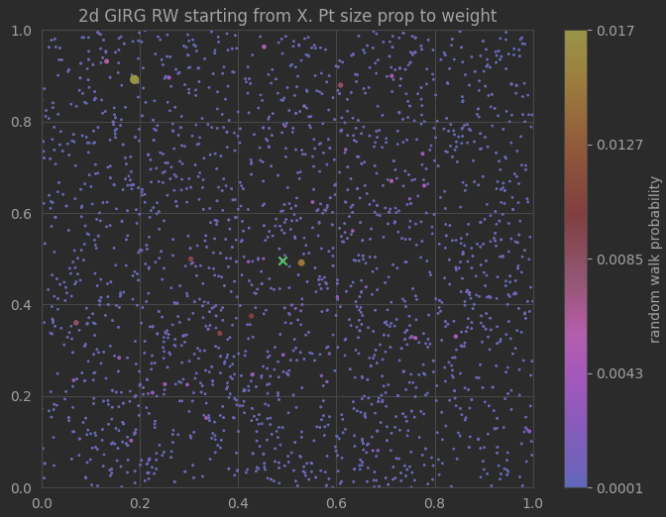
\includegraphics[width=\linewidth]{figures/2d_GIRG_RW.png}
    \caption{Naive approach: Large weight nodes (drawn with larger radii) get disproportionately more probability mass.}
  \end{subfigure}
  \hfill
  \begin{subfigure}{0.49\textwidth}
    \centering
    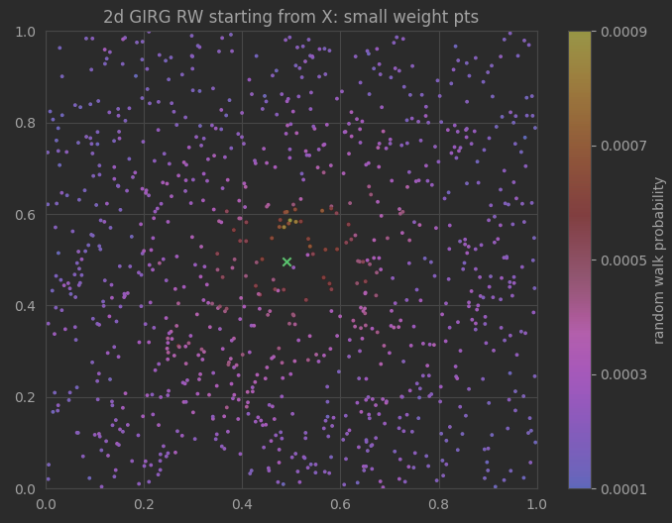
\includegraphics[width=\linewidth]{figures/2d_GIRG_RW_small_weights.png}
    \caption{Restriction of previous plot to nodes with smaller weights. Probability distribution looks more gaussian}
  \end{subfigure}

  \vspace{1em}

  \begin{subfigure}{0.49\textwidth}
    \centering
    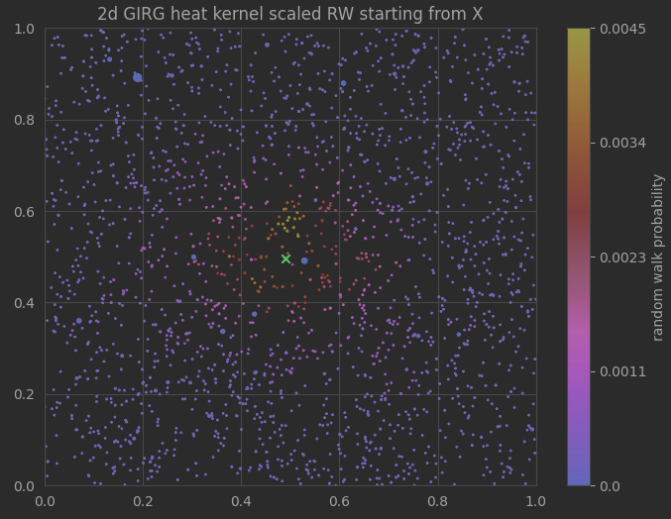
\includegraphics[width=\linewidth]{figures/2d_GIRG_heatkernelscaled_RW.png}
    \caption{Heat Kernel scaled edge weights using expected distance $W_{uv} = e^{-\hat{r}_{uv}^2}$. Helps to remove the large weight bias - perhaps a little too much.}
  \end{subfigure}
  \hfill
  \begin{subfigure}{0.49\textwidth}
    \centering
    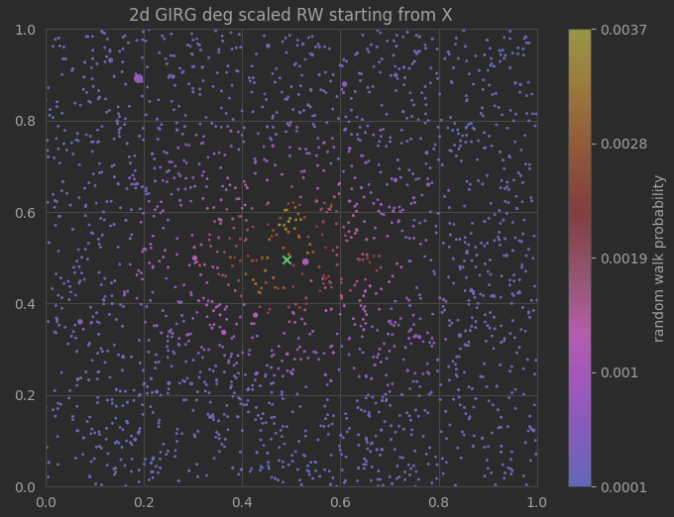
\includegraphics[width=\linewidth]{figures/2d_GIRG_degscaled_RW.png}
    \caption{Scaling transition probabilities by node degree $d_i^{-1}$  also removes the large weight bias.}
    \label{fig:diffmap_algo_comparisons_degscaled}
  \end{subfigure}
  \caption{6 step random walk diffusion cloud starting at the node marked with the green x, for three different (weightings) transition probability schemes. Graph generated from a 2d torus GIRG, whose true point locations give x and y axis.}
  \label{fig:diffmap_algo_comparisons}
  % \caption{Diffusion map eigenvalues (including $\lambda_1 = 1$) for a $n=2000, \tau=2.5, \alpha=1.3$ Cube GIRG with $d=1,2,3,4$ dimensions.}
  % \label{fig:cube_diffmaps_d1to4_evals}
\end{figure}



% % 
% The m-truncated diffusion map representation becomes the new r epresentation of nodes in the graph. The diffusion map is then a function $\R^n \to \R^m$. The first coordinate $\lambda_1$ is always $1$, corresponding to the stationary distribution of the random walk which all node diffusion maps converge to. This is useless for differentiating nodes and is hence dropped.

% Notably the transition matrix satisfies $M1 = 1$ since $\sum_j \frac{w_{ij}}{\deg(i)} = 1$, and it can be shown that it has eigenvalues $\lambda_1=1 \geq \lambda_2 \geq \lambda_3 \geq ...$.  





% Oh no $\vec{x}$.

% by the transition matrix $M = D^{-1}W$, where $D$ is the diagonal matrix with $D_{uu} = \sum_{v\in V} W_{uv}$ is the diagonal degree matrix, and $W_{uv}$ is the adjacency matrix, $W_{uv} = \begin{cases}1 & u \sim v \\0 & u \nsim v \end{cases}$. The matrix $S = D^{-1/2} W D^{-1/2}$ is a symmetrised version and hence is diagonalisable as $S = V \Lambda V^T$. Then the map $M = D^{-1/2} S D^{1/2} = D^{-1/2} V \Lambda (D^{1/2} V)^T = \Phi \Lambda \Psi^T$.

% In particular, starting at node $i$ (numbered $i=1,...,n$), the $t$th step diffusion cloud is $i \mapsto M^t_{ij} = (\Phi \Lambda^t \Psi^T)_{ij} = \sum_{k=1}^n \Phi_{ik} \lambda_k^t \Psi_{jk}$.

% So writing $\Phi = [\phi_1, \phi_2, ..., \phi_n]$ and $\Psi = [\psi_1, \psi_2, ..., \psi_n]$, we have that the $t$th step diffusion cloud is $i \mapsto \sum_{k=1}^n \phi_k(i) \lambda_k^t \vec{\psi}_k$. I.e. the diffusion map coordinate system is $\text{diffmap}_t(i) = (\lambda_2^t \phi_2(i), \lambda_3^t \phi_3(i), ..., \lambda_{d+1}^t \phi_{d+1}(i))$. The first coordinate is always $1$, it's the stationary distribution that all diffusion clouds converge to, so is discarded.

\section{Rescaling Points and Empirical Results}
If we have a graph $G$ which we know is generated from a $d$-dimensional GIRG, we can simply extract the $d$-truncated diffusion map coordinates of each node as an initial estimate for the original geometric location of the node. From \cref{sec:diff_map_geometry} we know the embedding should be roughly isometric up to a scale factor - so rescaling and shifting into the unit cube/torus is a first good step to make inter-point distances meaningful (even though this could be absorbed into the probability scaling constant $c$). There are also some other post processing steps that can be done to improve fit for real graphs.

\subsection{Inferring dimension $d$}
A first question is to choose the output dimension $d$ (truncation for the embedding) of the diffusion map, if the true geometric dimension $d$ of the input graph $G$ is unknown.

Diffusion maps actually present one way to infer the dimensionality by analysing the ordered sequence of eigenvalues $\lambda_2 < \lambda_3 < ...$. For example in \cref{fig:cube_diffmaps_d1to4_evals} we see that for graphs generated from cube GIRGs with dimension $d=1,2,3,4$, the diffusion map eigenvalue have a clear cutoff point after the first $d+1$ eigenvalues, with $\lambda_2, ..., \lambda_{d+1}$ being all approximately equal. Hence an eigenvalue cutoff can be used to infer geometric dimensionality of a graph - unfortunately messier real world graphs may not be so clear cut.

TODO plot some real graph eigenvalue plots?

% If there is a good cutoff point whereby the first $d$ eigenvalues are of similar large size, and the rest are much smaller, . This indeed works well for graphs synthetically generated from GIRGs, not so well on real world graphs.



\begin{figure}
  \centering

  \begin{subfigure}{0.49\textwidth}
    \centering
    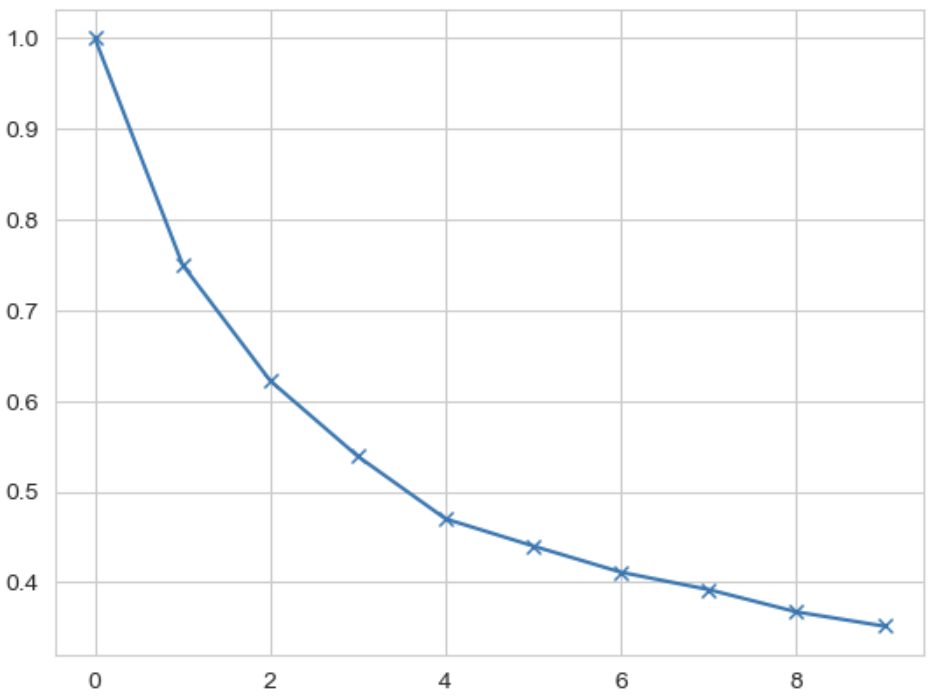
\includegraphics[width=\linewidth]{figures/diffmap_1d.png}
    \caption{$d=1$}
  \end{subfigure}
  \hfill
  \begin{subfigure}{0.49\textwidth}
    \centering
    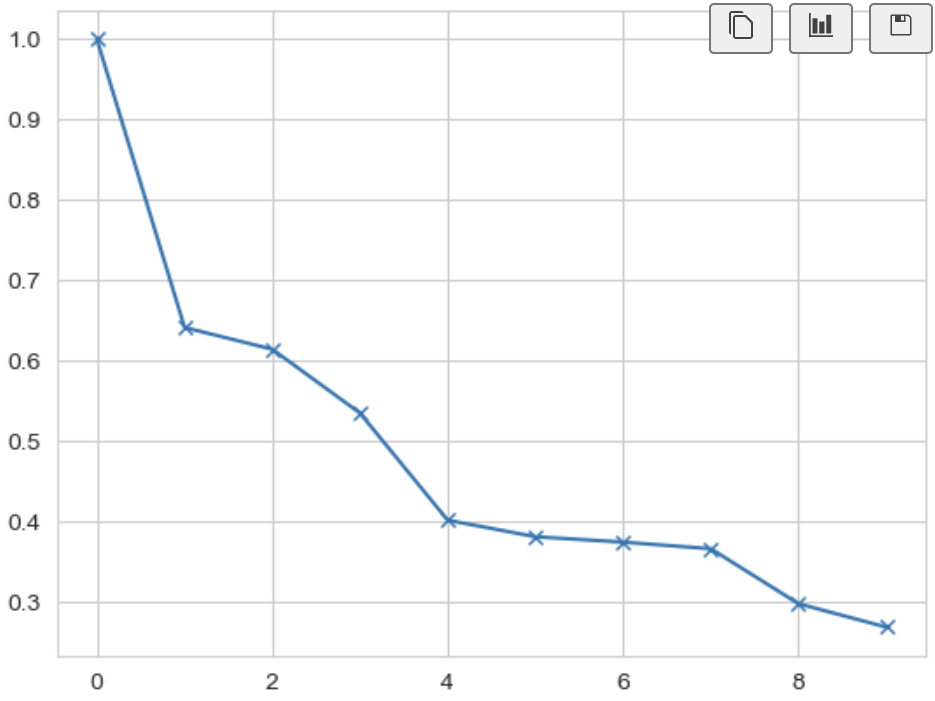
\includegraphics[width=\linewidth]{figures/diffmap_2d.png}
    \caption{$d=2$}
  \end{subfigure}

  \vspace{1em}

  \begin{subfigure}{0.49\textwidth}
    \centering
    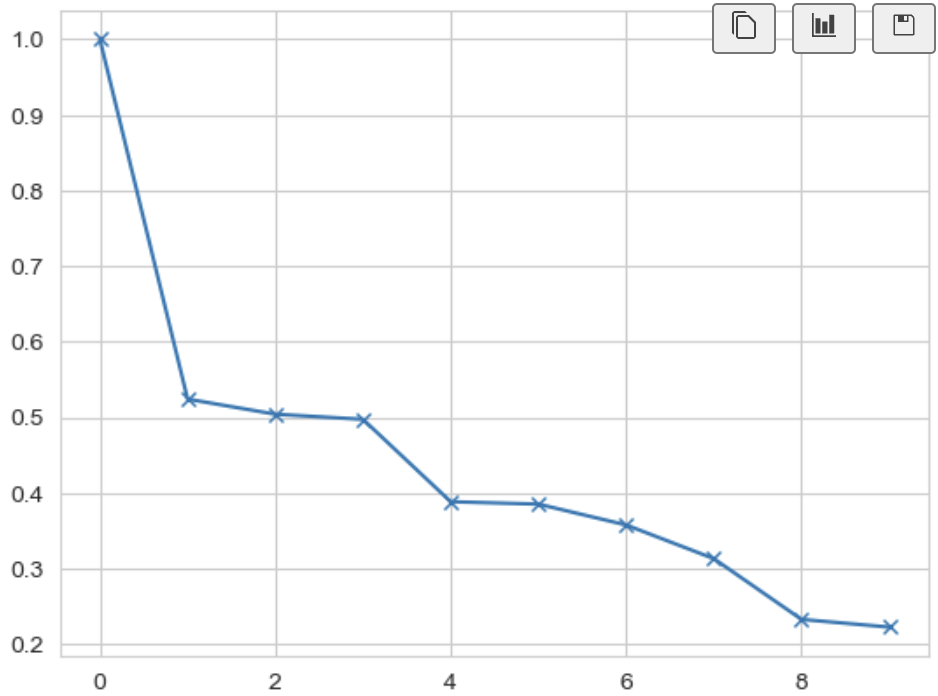
\includegraphics[width=\linewidth]{figures/diffmap_3d.png}
    \caption{$d=3$}
  \end{subfigure}
  \hfill
  \begin{subfigure}{0.49\textwidth}
    \centering
    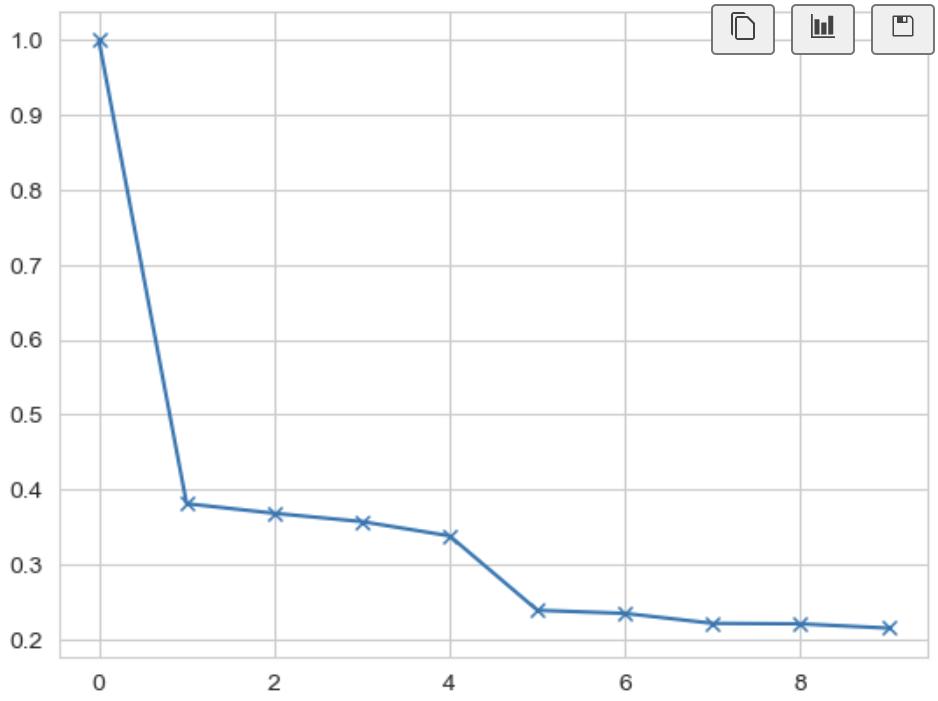
\includegraphics[width=\linewidth]{figures/diffmap_4d.png}
    \caption{$d=4$}
    \label{fig:cube_diffmaps_d4}
  \end{subfigure}

  \caption{Diffusion map eigenvalues (including $\lambda_1 = 1$) for a $n=2000, \tau=2.5, \alpha=1.3$ Cube GIRG with $d=1,2,3,4$ dimensions.}
  \label{fig:cube_diffmaps_d1to4_evals}
\end{figure}
\subsection{Rescaling/Shifting Diffusion Maps}
We see in \cref{fig:cube_diffmap_plots_d1and2} some raw $d=2$ truncated diffusion maps. When the underlying graph was a 2d square GIRG, the inferred points look indeed square like, whereas from a 1d GIRG we do at least get a (curved) line in 2d space.


In general the points will be centered around the origin, as all $\lambda_2, \lambda_3, ...$ eigenvalue eigenvectors will be orthogonal to the stationary distribution $\vec{\phi}_1 = k \vec{1}$ : they represent a deviation from the stationary distribution - e.g. for a node on the 1D line towards left end, it will need to put more diffusion probability on the left side nodes, and less on the right side nodes than the stationary distribution. The y-axis scale is small as $\lambda_2 < 1$, and is decreasing with $t$.


The 0 centering can easily be fixed to be more cube GIRG like by shifting the points $(\vec{x}_u)_i \gets (\vec{x}_u)_i + \min_v (\vec{x}_v)_i$.
If we are certain that the points should be distributed within the unit cube, then we can simply rescale separately along each dimension: $x \gets \frac{x - x_{\min}}{x_{\max} - x_{\min}}$.
If furthermore we're certain that the distribution within the unit cube should be relatively uniform, we can perform a coordinatewise "uniformify" procedure that replaces $(\vec{x}_u)_i$ with its percentile value compared with other $(\vec{x}_v)_i$. \cref{fig:diffmap_uniformed_vs_nonuniformed} shows the "uniformify" procedure in action. This helps to counteract the phenomenon of terribly different diffusion map scaling, whereby the majority of the graph which is well connected ends up highly bunched up, and a small number of outlying poorly connected nodes cover most of the embedding space. 

% Notably on real graphs where the truncated diff map coordinates are not guaranteed to be independently distributed, coordinatewise percentile mapping can lead to slightly odd results - see socfb-Amherst where there's a strong $x_1 = 1 - x_2$ correlation for small $x_1$. It's still a good improvement over the original non rescaled diffusion map.

% The decreasing diffusion map scaling can be see either as a bug or a feature. If we are certain that the points should be distributed within the unit cube, then we can simply rescale separately along each dimension: $x \gets \frac{x - x_{\min}}{x_{\max} - x_{\min}}$. If furthermore we're certain that the distribution within the unit cube should be relatively uniform, we can perform a coordinatewise "uniformify" procedure that replaces $(x_u)_i$ with its percentile value compared with other $(x_v)_i$. \cref{fig:diffmap_uniformed_vs_nonuniformed} shows the "uniformify" procedure in action. Notably on real graphs where the truncated diff map coordinates are not guaranteed to be independently distributed, coordinatewise percentile mapping can lead to slightly odd results - see socfb-Amherst where there's a strong $x_1 = 1 - x_2$ correlation for small $x_1$. It's still a good improvement over the original non rescaled diffusion map. 

% Critically since there is no guarantee that the scaling of diffusion map coordinates is the same as the original GIRG coordinates, using some kind of prior knowledge to rescale the diffusion map is important to yield geometric information with meaningful inter-point distances.

\begin{figure}
  \centering

  \begin{subfigure}{0.49\textwidth}
    \centering
    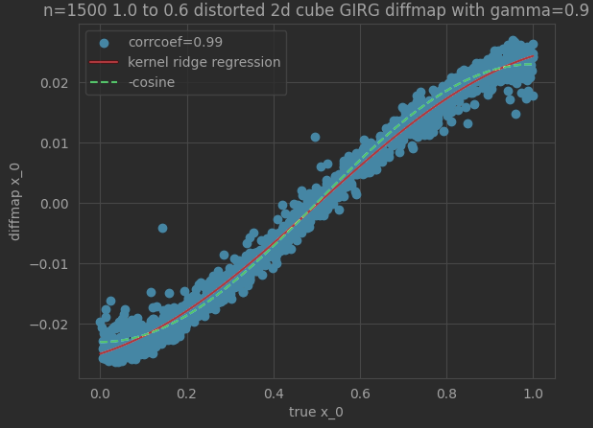
\includegraphics[width=\linewidth]{figures/2d_distorted_diffmap_plot_major.png}
    \caption{$d=1$}
    \label{fig:2d_distorted_major}
  \end{subfigure}
  \hfill
  \begin{subfigure}{0.49\textwidth}
    \centering
    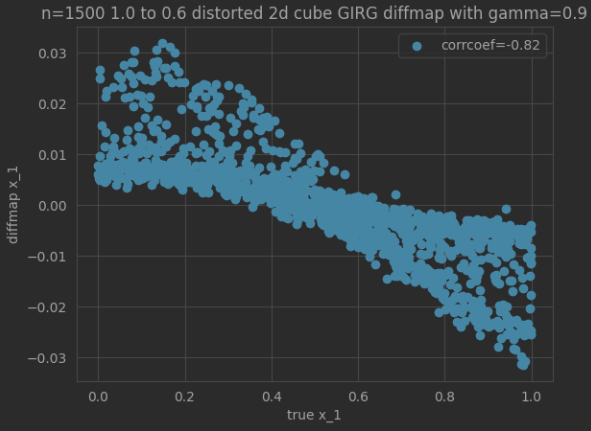
\includegraphics[width=\linewidth]{figures/2d_distorted_diffmap_plot_minor.png}
    \caption{$d=2$}
    \label{fig:2d_distorted_minor}
  \end{subfigure}


  \caption{Major and minor diff map against real}
  \label{fig:2d_distorted_major_minor}
\end{figure}


\paragraph{Rotated Points} One issue with diffusion maps as seen in \cref{fig:cube_diffmap_plots_d2}, the 2D GIRG's 2D-truncated diff map looks like a rotated square. While the diffusion map has successfully extracted geometric information from the graph, it's not done so in the original basis. This phenomenon can make rescaling/uniformifying to the unit cube a little questionable. 

One possible explanation is that as diffusion map is trying to maximise diffusion explainability, the long square diagonal has overall more diffusion along it. This is not very convincing though as there would then be less diffusion in the opposite corners. Even assuming no overall rotation bias, you're going to get a square rotated somewhere between $0$ and $45$ degrees.

\paragraph{Cuboidal (non-cube) GIRGs} However in practice, real graphs never have an equal balance in geometric dimension importance. This is easiest to understand with the example of a weighted euclidean norm setup, where it could be that a 2D GIRG's true 1st geometric dimension (between $[0, 1]$) is more important than its 2nd geometric dimension in influencing edge probabilities: $\norm{x - y} = \sqrt{a (x_1 - y_1)^2 + b(x_2 - y_2)^2}$.
The diffusion map is solving an eigenvalue problem that is like a maximsation of diffusion explainability. If $a > b$, then by maximisation the first diffusion map coordinate $\varphi_1(u)$ is likely to be very similar to $(\vec{x}_u)_1$. Only if $a=b$ is there no preference between $(\vec{x}_u)_1$ and $(\vec{x}_u)_2$, making a rotation possible.
Hence the points $(\varphi_1(u), \varphi_2(u))_{u \in V}$ are likely to end up as a rectangle, not a rotated square; the variation in first coordinate will be greater than in the second.

\cref{fig:2d_distorted_major} shows the 2d diff map embedding of such a distorted 2d cube GIRG. Note that the major coordinate is much easier to fit well, whereas the minor one has higher error (NB the diff map embedding of $x_2$ is negatively scaling with the true value which is fine - we can never guarantee same signs).
We also see that the $x_1$ diffusion map embedding doesn't have quite a linear relationship with the real locations - it looks more like a cosin wave like relationship - this actually makes sense as eigenfunctions of the laplacian operator on a cube look like sine waves.


In the light of potentially non equal coordinates, the relative $\lambda_2 > \lambda_3 > ...$ scaling can be seen as a feature not a bug, if the hypothesis space of generative graph models is to be expanded to cuboid (non-cube) GIRGs. In this case all coordinates of the diffusion map don't have to be all (non-homogeneously) rescaled to the range $[0, 1]$ and can rather be homogeneously rescaled to retain their relative size ratios.
This sheds new light on the horizontalness of the $\lambda_2, \lambda_3, \lambda_4, \lambda_5$ line segment in \cref{fig:cube_diffmaps_d4} as a testament to the underlying cube (non cuboid) GIRG that generated the graph.




% In this case, the diffusion map coordinates will have a larger scale for the $\lambda_2$ coordinate than the $\lambda_3$ coordinate, and the points will look like an elongated rectangle.

% the distance: $\norm{x - y} = \sqrt{a (x_1 - y_1)^2 + b(x_2 - y_2)^2}$. In this case, the diffusion map coordinates will have a larger scale for the $\lambda_2$ coordinate than the $\lambda_3$ coordinate, and the points will look like an elongated rectangle. The flatness of $\lambda_2, \lambda_3, \lambda_4, \lambda_5$ line segment in \cref{fig:cube_diffmaps_d4} is a testament to the cube (and non cuboidness) of the underlying GIRG that generated the graph.


% (relatively uniformly) distributed within the unit cube, then we can simply rescale separately along each dimension.
% A linear coordinatewise scaling $x \gets \frac{x - x_{\min}}{x_{\max} - x_{\min}}$ works, or more extremely a coordinatewise "uniformify" procedure that replaces $(x_u)_i$ with its percentile value compared with other $(x_v)_i$.
% In \cref{fig:diffmap_uniformed_vs_nonuniformed} we see uniformified versions of a generated 2D GIRG, and the socfb-Amherst41 graph.

% Seen as a feature, the relatively different scaling allows as a natural correction to the potential non equivalence of different dimensions. For instance in a weighted euclidean norm setup, it could be that a 2D GIRG's true 1st geometric dimension (between $[0, 1]$) is much more important than its 2nd geometric dimension in determining the distance: $\norm{x - y} = \sqrt{a (x_1 - y_1)^2 + b(x_2 - y_2)^2}$. In this case, the diffusion map coordinates will have a larger scale for the $\lambda_2$ coordinate than the $\lambda_3$ coordinate, and the points will look like an elongated rectangle. The flatness of $\lambda_2, \lambda_3, \lambda_4, \lambda_5$ line segment in \cref{fig:cube_diffmaps_d4} is a testament to the cube (and non cuboidness) of the underlying GIRG that generated the graph. 


% TODO put in some eigenvalue plots

\begin{figure}
    \centering

    \begin{subfigure}{0.49\textwidth}
      \centering
      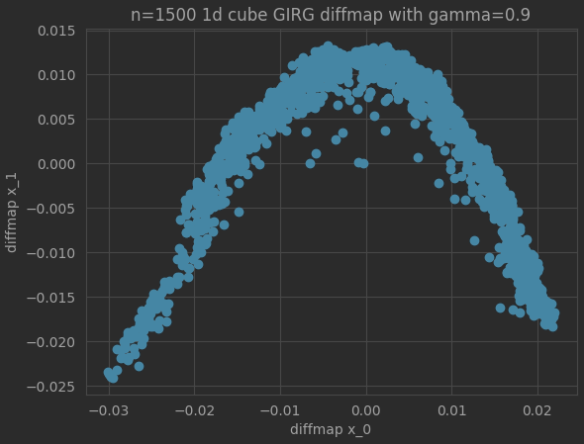
\includegraphics[width=\linewidth]{figures/1d_GIRG_diffmap.png}
      \caption{$d=1$}
      \label{fig:sub1}
    \end{subfigure}
    \hfill
    \begin{subfigure}{0.49\textwidth}
      \centering
      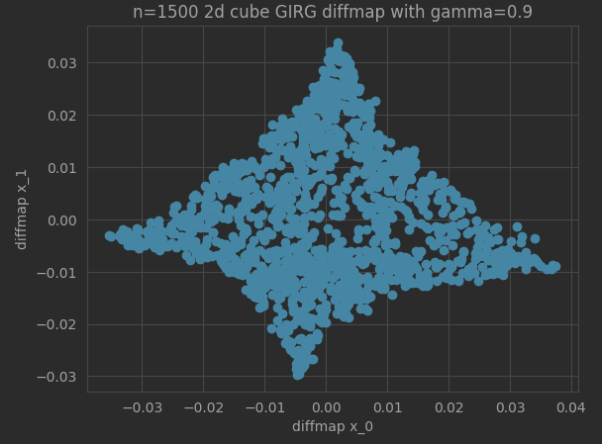
\includegraphics[width=\linewidth]{figures/2d_GIRG_diffmap.png}
      \caption{$d=2$}
      \label{fig:cube_diffmap_plots_d2}
    \end{subfigure}

  
    \caption{Diffusion map scatter plot of the first two extracted coordinates from 1d and 2d GIRGs.}
    \label{fig:cube_diffmap_plots_d1and2}
\end{figure}


\begin{figure}
    \centering

    \begin{subfigure}{0.49\textwidth}
      \centering
      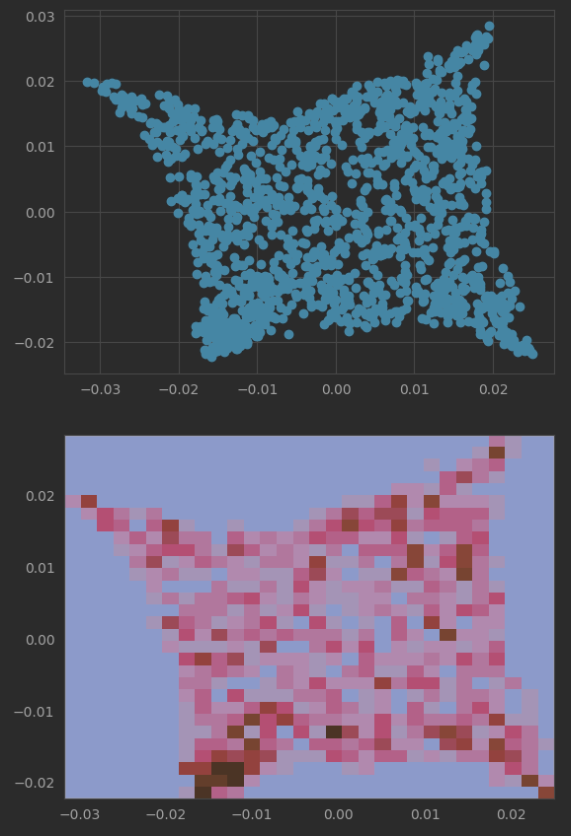
\includegraphics[width=\linewidth]{figures/diffmap_plot_nonuniformed.png}
      \caption{2d GIRG non-uniformed}
      \label{fig:sub1}
    \end{subfigure}
    \hfill
    \begin{subfigure}{0.49\textwidth}
      \centering
      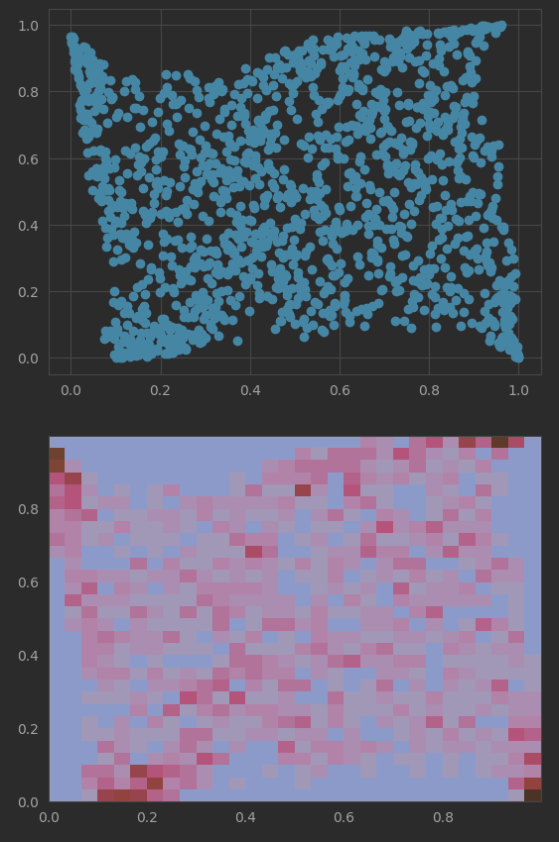
\includegraphics[width=\linewidth]{figures/diffmap_plot_uniformed.png}
      \caption{2d GIRG uniformed}
      \label{fig:sub2}
    \end{subfigure}
  
    \vspace{1em}
  
    \begin{subfigure}{0.49\textwidth}
      \centering
      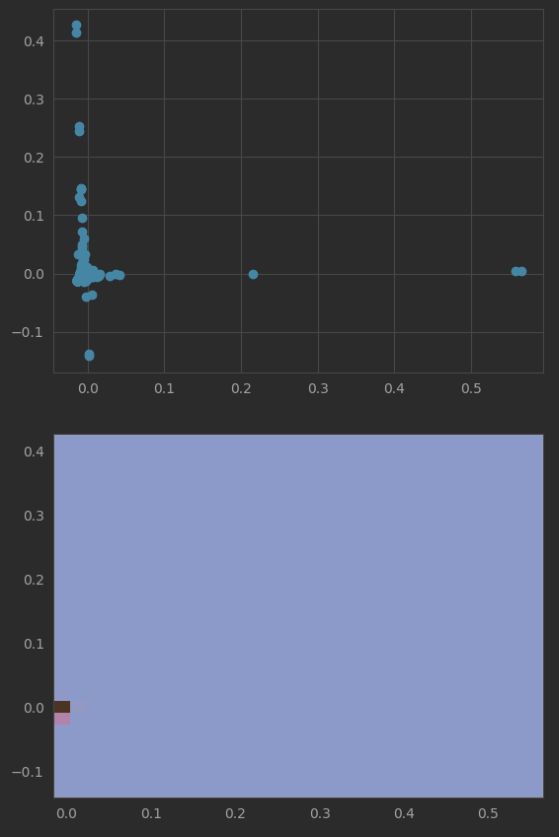
\includegraphics[width=\linewidth]{figures/real_diffmap_plot_nonuniformed.png}
      \caption{socfb-Amherst41 non-uniformed}
      \label{fig:sub3}
    \end{subfigure}
    \hfill
    \begin{subfigure}{0.49\textwidth}
      \centering
      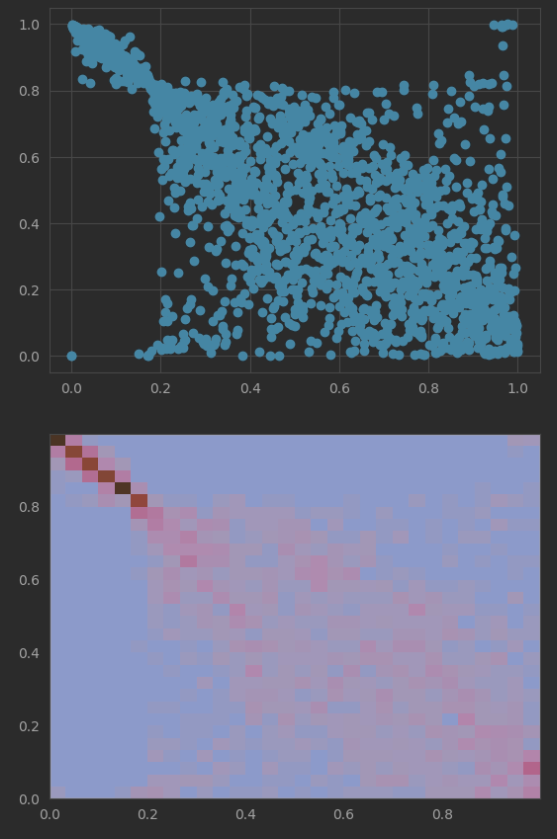
\includegraphics[width=\linewidth]{figures/real_diffmap_plot_uniformed.png}
      \caption{socfb-Amherst41 uniformed}
      \label{fig:sub4}
    \end{subfigure}
  
    \caption{Diffusion map scatter plot of the first two extracted coordinates, with and without using an additional uniform square remapping}
    \label{fig:diffmap_uniformed_vs_nonuniformed}
\end{figure}


% \begin{figure}
%   \centering

%   \begin{subfigure}{\textwidth}
%     \centering
%     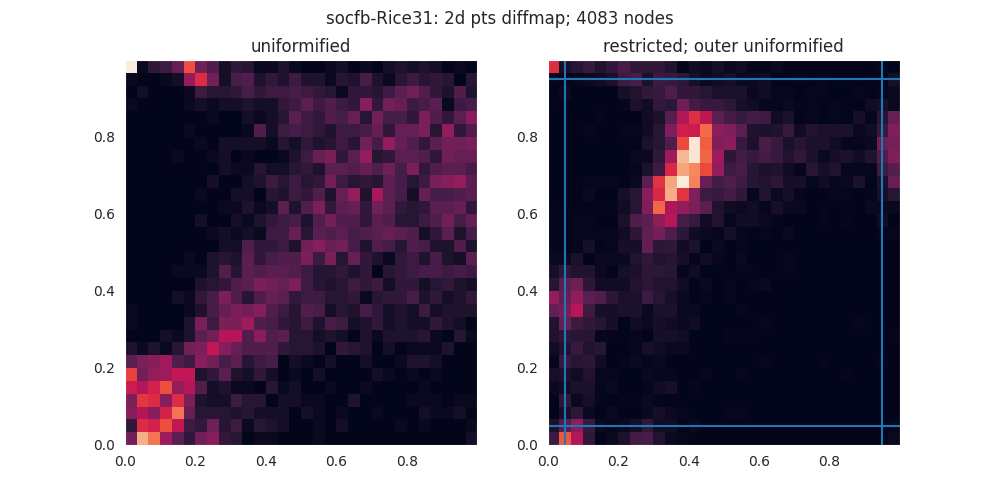
\includegraphics[width=\linewidth]{figures/socfb-Rice31_2ddiffmap_unif_vs_restrict.png}
%     % \label{fig:sub1}
%   \end{subfigure}

%   \vspace{1em}
%   \begin{subfigure}{\textwidth}
%     \centering
%     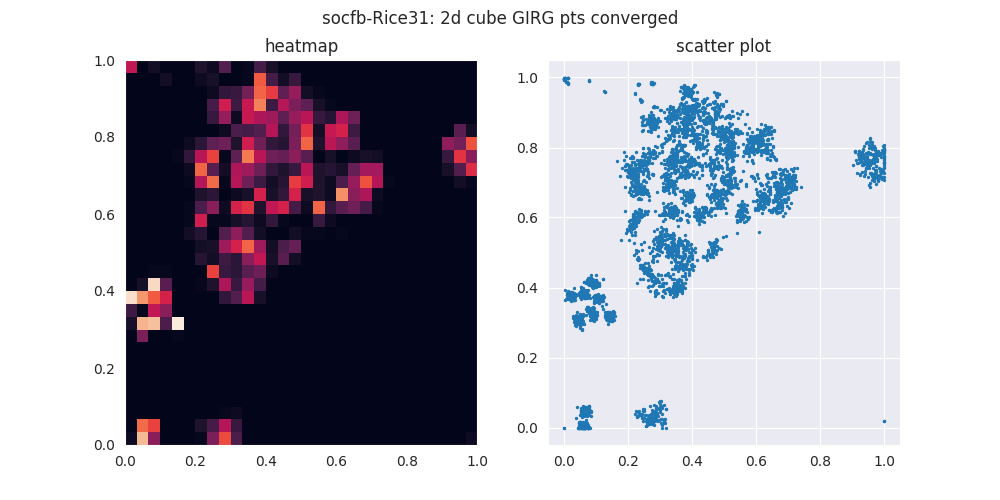
\includegraphics[width=\linewidth]{figures/socfb-Rice31_2d_cube_GIRG_converged.png}
%     % \label{fig:sub1}
%   \end{subfigure}

%   \vspace{1em}
  
% \end{figure}
% \begin{figure}
%   \begin{subfigure}{\textwidth}
%     \centering
%     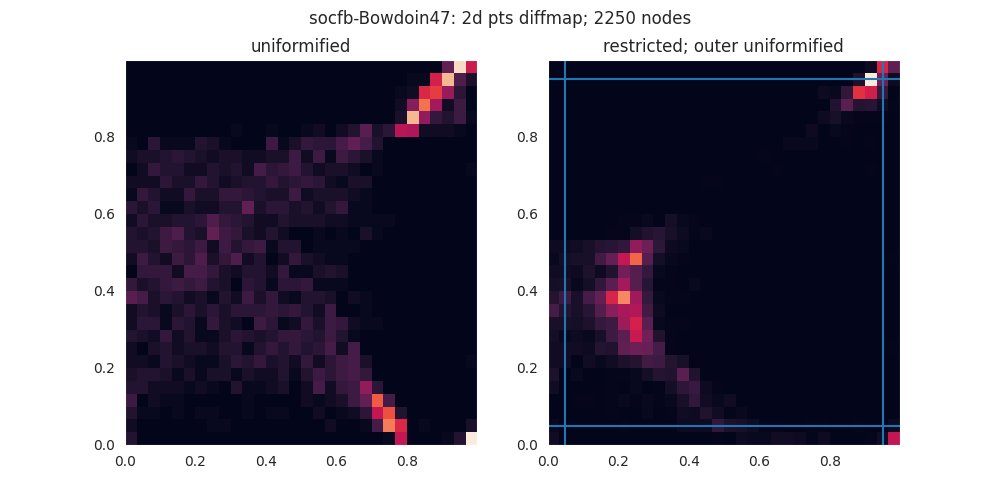
\includegraphics[width=\linewidth]{figures/socfb-Bowdoin47_2ddiffmap_unif_vs_restrict.png}
%     % \label{fig:sub1}
%   \end{subfigure}

%   \vspace{1em}
%   \begin{subfigure}{\textwidth}
%     \centering
%     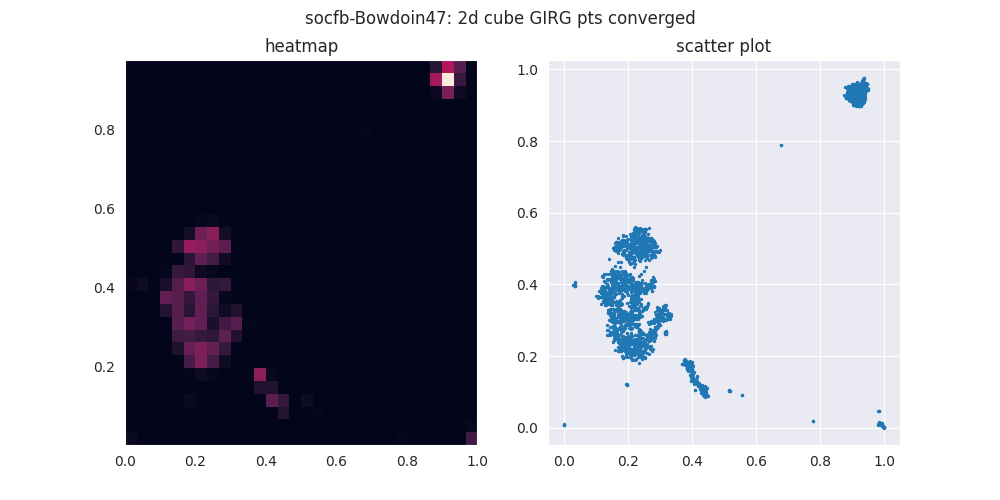
\includegraphics[width=\linewidth]{figures/socfb-Bowdoin47_2d_cube_GIRG_converged.png}
%     % \label{fig:sub1}
%   \end{subfigure}

% \end{figure}


% \begin{figure}
%   \begin{subfigure}{\textwidth}
%     \centering
%     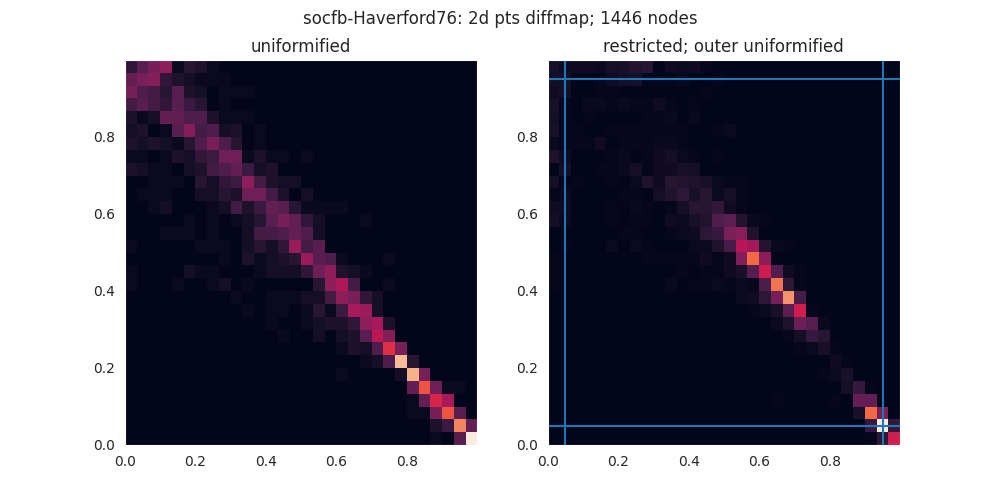
\includegraphics[width=\linewidth]{figures/socfb-Haverford76_2ddiffmap_unif_vs_restrict.png}
%     % \label{fig:sub1}
%   \end{subfigure}

%   \vspace{1em}
%   \begin{subfigure}{\textwidth}
%     \centering
%     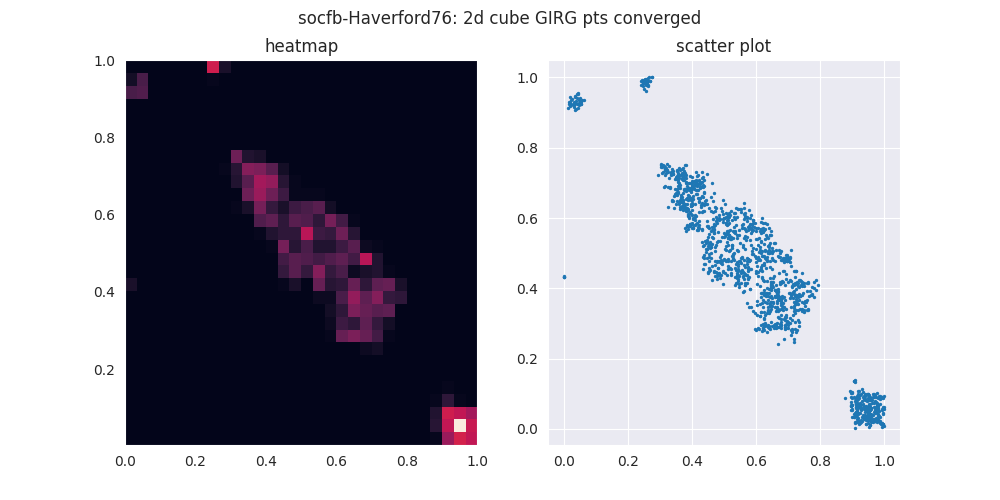
\includegraphics[width=\linewidth]{figures/socfb-Haverford76_2d_cube_GIRG_converged.png}
%     % \label{fig:sub1}
%   \end{subfigure}


%   \caption{two methods for rescaling/shifting diffusion maps into the cube - done here for d=2 truncations. The blue lines for the restricted version show the border at which points are outer uniformified.}
%   \label{fig:uniformifed_vs_restricted_rescaling}
% \end{figure}


\begin{figure}
  \begin{subfigure}{0.47\textwidth}
    \centering
    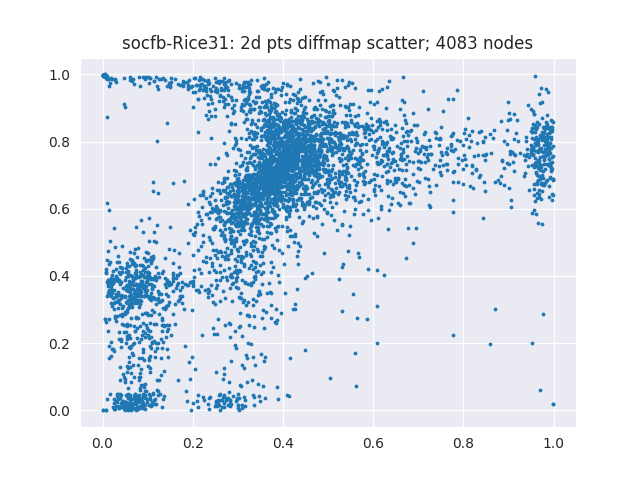
\includegraphics[width=\linewidth]{figures/socfb-Rice31_2ddiffmap_restrict_scatter.png}
    % \label{fig:sub1}
  \end{subfigure}
  \hfill
  \begin{subfigure}{0.47\textwidth}
    \centering
    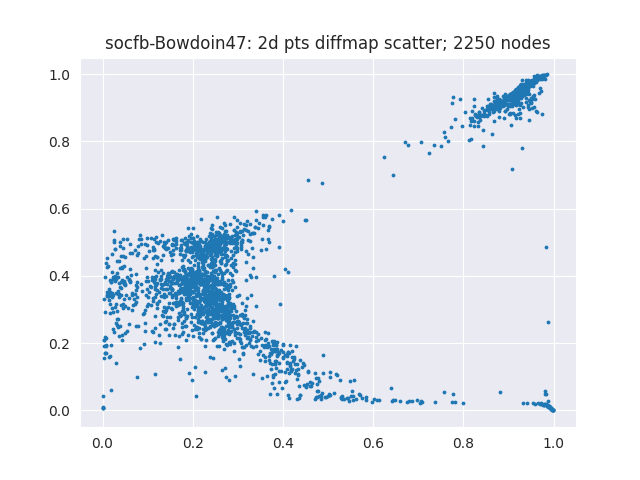
\includegraphics[width=\linewidth]{figures/socfb-Bowdoin47_2ddiffmap_restrict_scatter.png}
    % \label{fig:sub1}
  \end{subfigure}


  \caption{the diffmaps (here 2d, restricted and outer uniformified) don't have much point clustering - it's more higher diffusion level than caring so much about individual edges like in the converged case}
  \label{fig:uniformifed_vs_restricted_rescaling}
\end{figure}



\paragraph{Toroidal GIRGs} Interestingly Toroidal GIRGs are differentiated from Cube GIRGs in that the diffusion map requires $2d$ coordinates to capture the Torus geometry instead of just $d$ for the cube. The natural diffusion map of a 1D Torus GIRG ends up being a 2D circle about the origin; 2 larger eigenvalues $\lambda_2, \lambda_3$ are necessary. 


% A final issue with diffusion maps is that points seem to end up concentrated in corners/edges. My hypothesis is that this is because e.g. on a 1D line segment, it's hard to distinguish somewhat left and very left points - in the end the diffusion cloud bias is still just left leaning. Not sure how much of a problem this is.

\paragraph{Restricted Rescaling} This method works to bias less towards a uniformly distributed prior while still mapping points into a reasonable geometric space.
Empirically, the diffusion map coordinates of the facebook graphs often have $\geq 90\%$ of the nodes concentrated in a small parcel, with only a few nodes having extremely far out locations.
This defeats the simple rescaling method of $x \gets \frac{x - x_{\min}}{x_{\max} - x_{\min}}$ as most nodes will end up very tightly packed - however if we hit all the points with a uniformify procedure hammer, we will lose the more subtle geometry picked up by the diffusion map within the highly connected central parcel.

Instead we only rescale the central nodes: those whose joint coordinate-wise percentiles lie in $[5\%, 95\%]^d$.
These nodes are linearly scaled to the $[0.05, 0.95]^d$ cube. Finally the outlying nodes are percentile rescaled (non-linearly) to the upper/lower cube margins.
This method is shown in comparison for a few graphs in \cref{fig:uniformifed_vs_restricted_rescaling}


TODO 

- fuller analysis of different diffmap modes: 'uniformify', 'cubify' and 'cuboidify', comparing performance on real life and synthetic graphs

- presentation of the small degree stochastic walk tweak which improves diffusion map performance:
\begin{verbatim}
# Empirically this gamma seems to work well. 
# It discourages taking edges to popular nhbs.
gamma = 0.9
M_tilde = scipy.sparse.diags(1 / D) @ A @ scipy.sparse.diags(D ** (-gamma))
M_tilde = scipy.sparse.diags(np.array(1 / M_tilde.sum(axis=-1)).squeeze()) @ M_tild
\end{verbatim}

- is it true that diffusion map tends to cluster representations edges rather than being more uniform? Empricially seems to happen in 2D but not 1D?

